% Chapter 4: Design and Implementation

\chapter{Diseño e implementación} % Main chapter title

\label{Chapter4} % Reference

%----------------------------------------------------------------------------------------

\section{Arquitectura de seguridad}

%----------------------------------------------------------------------------------------

\section{Arquitectura del software}

Para explicar la arquitectura software de la aplicación, esta sección va a estar dividida en varios
prototipos que se han desarrollado:

\subsection{Shatter 0.1}

El primer prototipo de la aplicación se desarrolló enteramente en Java, usando para ello el entorno
de desarrollo Eclipse. Esta primera versión buscaba poder dividir un fichero en varios fragmentos
de un tamaño dado, y luego poder recomponerlo. Para ello se implementaron algunas clases:

\begin{itemize}
  \item \keyword{Slice} -- Un Slice es uno de los fragmentos en los que un
  fichero original se ha dividido. Está formado por una cabecera (Header) y un
  array de bytes en el que se almacena el contenido de una partición del fichero.
  (Figura~\ref{fig:Slice_Header})

  \item \keyword{Header} -- En esta clase se almacenan los metadatos de los
  Slices. Se guardan datos como el orden de los Slices, el número total de Slices
  para un fichero, un ID para la sesión\footnote{En esta primera iteración de la
  aplicación, el ID para identificar la sesión era un resumen Hash del fichero.},
  el tamaño original del fichero y una firma de los datos a los que acompaña la cabecera.
  (Figura~\ref{fig:Slice_Header})

  \item \keyword{Slicer} -- Esta clase es la \emph{fábrica} de Slices. Recibe
  un fichero, un tamaño de bloque y un ID para identificar la sesión. Lee del
  fichero bloques del tamaño indicado hasta alcanzar el EOF y genera un Slice
  para cada uno de ellos, con una cabecera distinta. (Figura~\ref{fig:Assembler})

  \item \keyword{Composer} -- Si el anterior recibía un fichero y generaba Slices,
  éste recibe Slices y devuelve un fichero compuesto. Lee uno a uno los Slices
  que recibe, prestando especial atención a sus cabeceras y si detecta que
  alguno falta genera un log de errores. (Figura~\ref{fig:Assembler})
\end{itemize}

Al tratarse de un prototipo bastante sencillo, no dió muchos problemas, se
alcanzaron fácilmente los objetivos buscados.

\begin{figure}[ht]
  \centering
  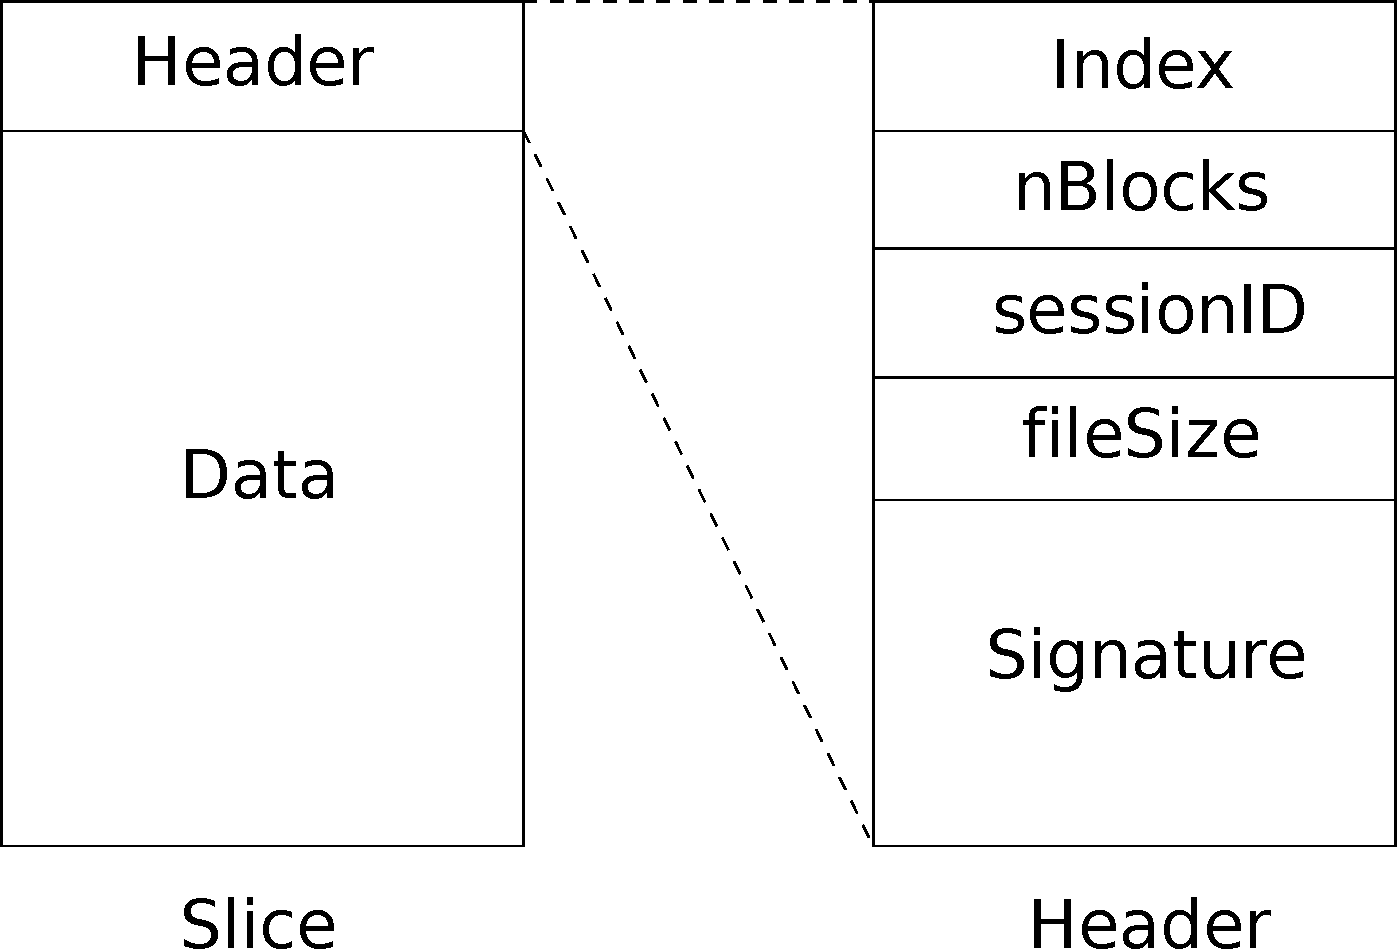
\includegraphics[scale=0.4]{Figures/Slice_Header}
  \decoRule
  \caption[Slice - Header]{Esquema general de las clases Slice y Header}
  \label{fig:Slice_Header}
\end{figure}

\begin{figure}[ht]
  \centering
  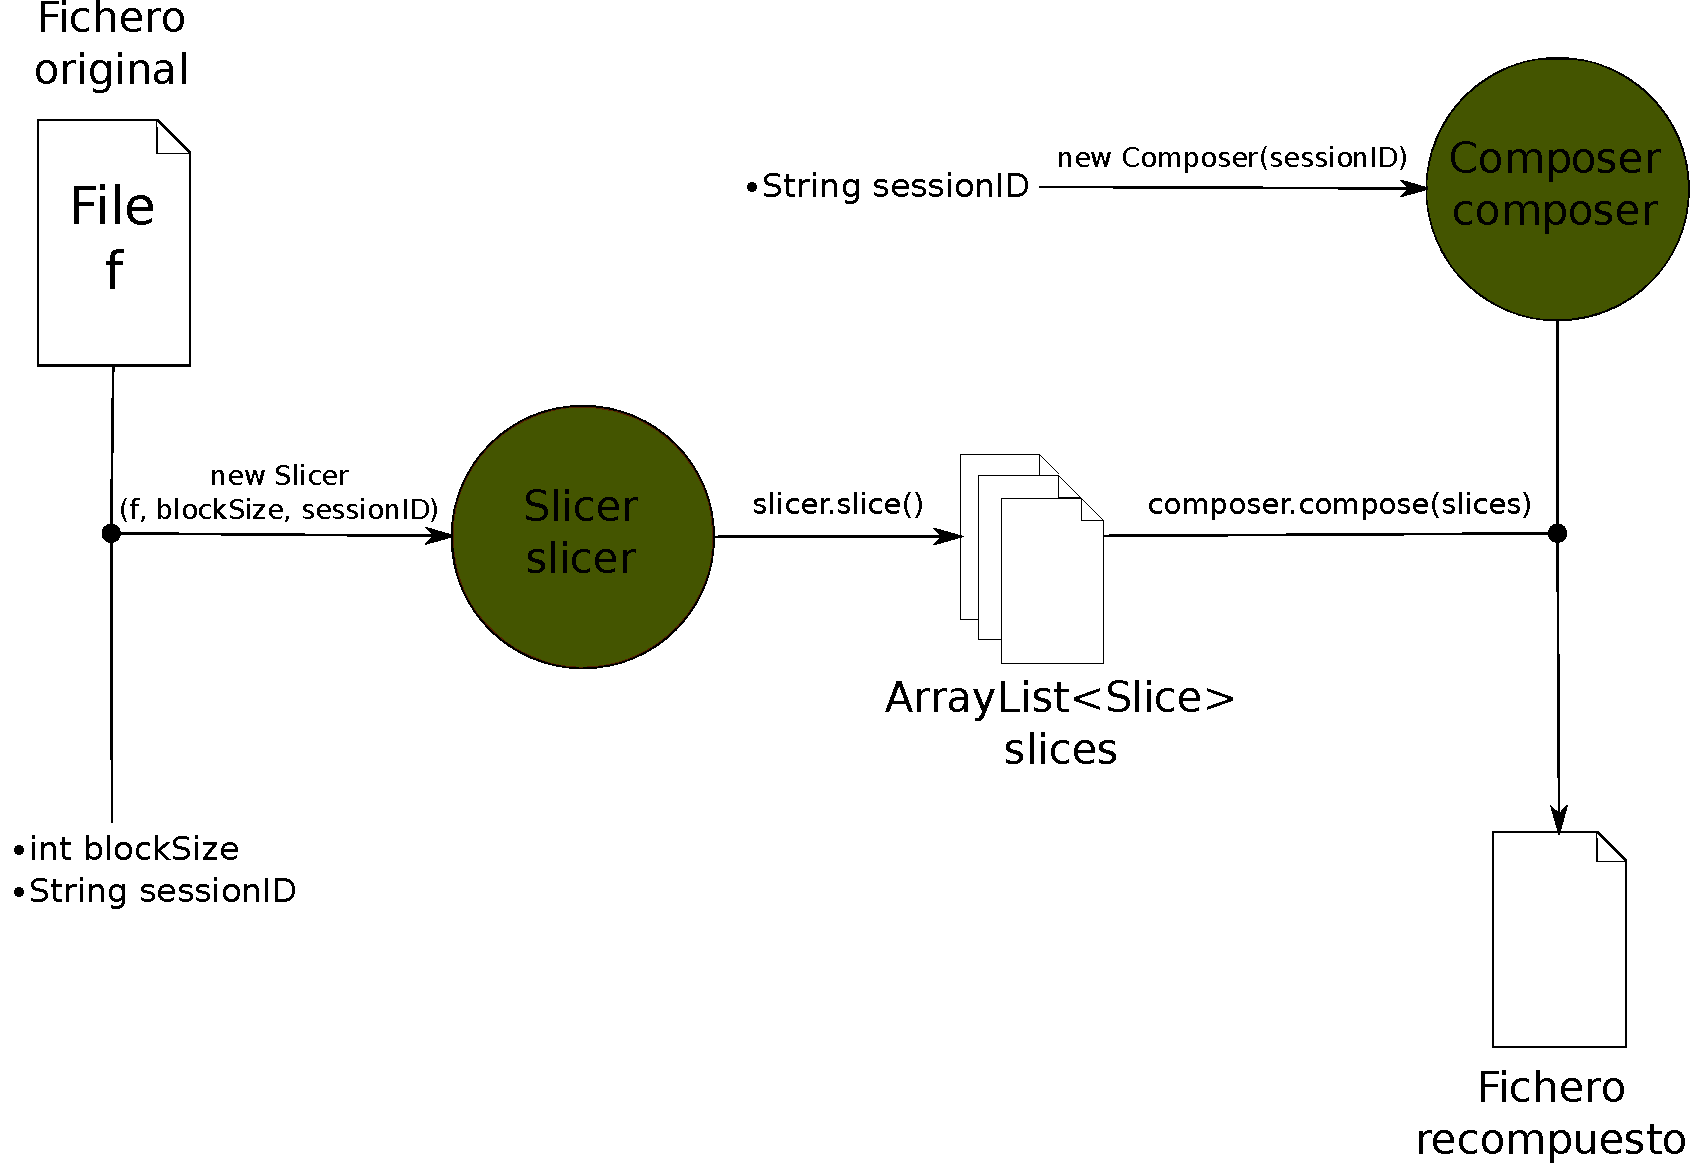
\includegraphics[scale=0.5]{Figures/Assembler}
  \decoRule
  \caption[Slicer - Composer]{Esquema general del Slicer y el Composer}
  \label{fig:Assembler}
\end{figure}
